% =====================================================================
%  AI & Applied Engineering - Lab 3: Multi-Stage AI Workflow Across UX Types
%  Resubmission
%
%  Compiles with pdflatex (twice, for the table of contents):
%      pdflatex lab3-multi-stage-ai-workflow.tex
%      pdflatex lab3-multi-stage-ai-workflow.tex
%  Or open this file in Overleaf and press Recompile.
% =====================================================================
\documentclass[11pt,a4paper]{article}

\usepackage[T1]{fontenc}
\usepackage[utf8]{inputenc}
\usepackage{lmodern}
\usepackage[english]{babel}
\usepackage[a4paper,margin=2.4cm]{geometry}

\usepackage{booktabs}
\usepackage{tabularx}
\usepackage{longtable}
\usepackage{array}
\usepackage{enumitem}
\usepackage{graphicx}
\usepackage{xcolor}
\usepackage{listings}
\usepackage{caption}
\usepackage{titlesec}
\usepackage{tikz}
\usetikzlibrary{arrows.meta,positioning,fit,backgrounds}
\usepackage[hidelinks]{hyperref}

% ---------------------------------------------------------------------
%  Styling
% ---------------------------------------------------------------------
\definecolor{accent}{HTML}{1F4E79}
\definecolor{codebg}{HTML}{F5F6F8}
\definecolor{codeframe}{HTML}{D8DCE2}
\definecolor{good}{HTML}{1B6B3A}
\definecolor{bad}{HTML}{A22C22}
\definecolor{warn}{HTML}{8A6100}
\definecolor{chatc}{HTML}{2E5E8C}
\definecolor{idec}{HTML}{6B4E9E}
\definecolor{clic}{HTML}{1B6B3A}

\hypersetup{
  colorlinks=true,
  linkcolor=accent,
  urlcolor=accent,
  pdftitle={Multi-Stage AI Workflow Across UX Types},
  pdfauthor={Katy Great Adonai}
}

\titleformat{\section}{\color{accent}\Large\bfseries}{\thesection}{0.7em}{}
\titleformat{\subsection}{\color{accent}\large\bfseries}{\thesubsection}{0.7em}{}
\titleformat{\subsubsection}{\bfseries}{\thesubsubsection}{0.7em}{}

\captionsetup{font=small,labelfont={bf,color=accent}}

\newcolumntype{L}[1]{>{\raggedright\arraybackslash}p{#1}}

\lstdefinestyle{plain}{
  basicstyle=\ttfamily\scriptsize,
  backgroundcolor=\color{codebg},
  frame=single,
  rulecolor=\color{codeframe},
  framesep=5pt,
  breaklines=true,
  columns=fullflexible,
  keepspaces=true,
  showstringspaces=false
}
\lstdefinestyle{java}{
  style=plain,
  language=Java,
  keywordstyle=\color{accent}\bfseries,
  commentstyle=\color{black!55}\itshape,
  stringstyle=\color{good}
}
\lstdefinestyle{json}{
  style=plain,
  literate=*{:}{{\textcolor{accent}{:}}}{1}
}
\lstset{style=plain}

\newcommand{\code}[1]{\texttt{\small #1}}
\newcommand{\ran}{\textcolor{good}{\textbf{EXECUTED}}}
\newcommand{\notran}{\textcolor{bad}{\textbf{NOT RUN}}}
\newcommand{\partly}{\textcolor{warn}{\textbf{PARTIAL}}}

\setlist[itemize]{leftmargin=1.4em,itemsep=2pt,topsep=3pt}
\setlist[enumerate]{leftmargin=1.6em,itemsep=2pt,topsep=3pt}

% =====================================================================
\begin{document}

\begin{titlepage}
\centering
\vspace*{2.2cm}

{\color{accent}\Huge\bfseries Multi-Stage AI Workflow\par}
\vspace{0.4cm}
{\color{accent}\Huge\bfseries Across UX Types\par}
\vspace{0.8cm}
{\LARGE AI \& Applied Engineering --- Lab 3\par}
\vspace{0.3cm}
{\large Resubmission\par}

\vspace{1.6cm}
\rule{0.75\textwidth}{1pt}\par
\vspace{0.7cm}
{\LARGE\bfseries Chat $\rightarrow$ IDE $\rightarrow$ CLI\par}
\vspace{0.35cm}
{\large Executed against \code{student-task-manager}, a real Java 21 codebase\par}
\vspace{0.7cm}
\rule{0.75\textwidth}{1pt}\par

\vspace{2.0cm}
{\large\bfseries Katy Great Adona\"i\par}
\vspace{0.25cm}
{\large AmaliTech Training --- DEG Apprenticeship, Java Backend\par}

\vspace{1.4cm}
{\large\textbf{Repository:} \url{https://github.com/g1kdo/student-task-manager}\par}
{\normalsize Branch \code{feature/task-due-dates}\par}

\vspace{0.9cm}
\begin{minipage}{0.86\textwidth}
\small\centering
\textbf{What changed since the first submission.} The first submission was a
design with no execution behind it: no repository, no prototype, and a
self-assessment that offered a mock transcript as ``objective proof the
artifact functions end-to-end''. That claim was wrong and is withdrawn.
This document reports only what was actually run, names the tool and operator
for each stage, and points every claim at a captured artefact. Section~4 states
plainly which stages executed and which did not.
\end{minipage}

\vfill
{\large 4 September 2026\par}
\end{titlepage}

\tableofcontents
\newpage

% =====================================================================
\section{Problem statement}

\code{student-task-manager} is a Java 21 console application with a small,
deliberately layered design: \code{ConsoleApp} renders and reads input,
\code{TaskManager} owns the rules and the task list, \code{Task} guards its own
invariants. At the point this workflow began it had 69 passing tests, 92.3\,\%
line coverage and a CI pipeline enforcing a coverage floor.

The feature put through the workflow is due dates:

\begin{quote}
\itshape
Let students give a task a due date so they can tell what's urgent. The due
date is optional. If they want reminding, we need to know how many days ahead
--- but a reminder makes no sense on a task with no due date. Don't let them
add the same task twice; tell them it already exists instead of silently adding
a duplicate. And when they list tasks, show which ones are overdue, which are
due today, and which are still upcoming.
\end{quote}

\subsection{Why this feature, and not a toy}

A workflow that only ever runs against a scratch project proves nothing about
whether it survives contact with real code. Four properties made this feature
worth chaining tools over:

\begin{enumerate}
  \item \textbf{A conditional contract rule.} \code{remindBeforeDays} is
        meaningful only when \code{dueDate} is present. Conditional
        requirement is trivial to state in prose and easy to get wrong in
        code, which makes it a real test of the hand-off fidelity between
        stages.
  \item \textbf{A conflict rule.} Rejecting a duplicate rather than silently
        adding it --- the console analogue of returning HTTP 409.
  \item \textbf{Derived state with genuine branching.} \code{OVERDUE} /
        \code{DUE\_TODAY} / \code{UPCOMING} / \code{NONE} is computed, never
        stored, and has boundaries either side of ``today'' that a
        return-value-only test can pass straight through.
  \item \textbf{It lands in an existing, already-green codebase.} The workflow
        had to produce an additive result that kept 69 tests passing and the
        coverage gate satisfied --- not a plausible-looking result on a
        throwaway repository.
\end{enumerate}

Point 4 is the substantive difference from the first submission. The original
design targeted \code{shopfront-api}, a Python service that did not exist; this
one targets a repository with a commit history, a CI pipeline and a coverage
gate that can all reject bad work.

% =====================================================================
\section{Tool selection and UX-to-stage fit}

Each stage uses the UX type that has an unfair advantage for that kind of work,
and hands off a machine-parseable artefact rather than prose.

\begin{table}[h]
\centering
\small
\begin{tabularx}{\textwidth}{@{}p{1.7cm} p{1.3cm} p{2.5cm} X@{}}
\toprule
\textbf{Stage} & \textbf{UX type} & \textbf{Tool used} & \textbf{Why this UX wins here} \\
\midrule
1. Design \& draft
  & \textcolor{chatc}{\textbf{Chat}}
  & Claude Opus 5 (Claude desktop app)
  & Chat is a \emph{reasoning canvas}. No filesystem, no premature edits ---
    which suits divergent design work: negotiating the contract, arguing the
    edge cases (duplicate semantics, whether a past due date is an error), and
    producing a self-contained draft. The wide thinking surface of chat beats
    an IDE when the artefact does not exist yet. \\
\addlinespace
2. Ground \& test
  & \textcolor{idec}{\textbf{IDE}}
  & GitHub Copilot, Agent mode, in VS Code
  & The IDE UX is \emph{repository-aware}. It reads the real
    \code{Task.java} and \code{TaskManager.java}, the actual import graph and
    the existing naming and Javadoc conventions. Its strength is grounded,
    multi-file edits --- placing the draft into the codebase as it is, not as
    the chat imagined it. Inline diffs give a fast approve/reject loop. \\
\addlinespace
3. Verify \& commit
  & \textcolor{clic}{\textbf{CLI}}
  & Claude Code
  & The CLI UX is an \emph{agentic executor with a real shell}. It runs
    \code{mvnw clean verify}, reads the failures, self-heals, and then reads the
    actual \code{git diff --staged} to author a truthful commit message. Chat
    cannot run your test suite; the IDE runs it awkwardly. The terminal is the
    native home of \emph{execute, observe, react}. \\
\bottomrule
\end{tabularx}
\caption{Stage-to-UX fit. Each tool is used only where its UX has an advantage,
and each hands off a parseable artefact --- a Markdown file, the git working
tree, a commit --- which is what makes the bridges frictionless.}
\end{table}

\subsection{The bridges carry no vendor}

Every hand-off rides on a universal primitive, which is what makes the design
tool-agnostic rather than merely claiming to be:

\begin{table}[h]
\centering
\small
\begin{tabularx}{\textwidth}{@{}l l X@{}}
\toprule
\textbf{Bridge} & \textbf{Primitive} & \textbf{What crosses it} \\
\midrule
1 $\rightarrow$ 2 & A file in the repository & Artifact A written to \code{docs/features/task-due-dates.md}. The IDE reads it with a file reference; nothing is pasted into code. \\
2 $\rightarrow$ 3 & The git working tree & Nothing is copied at all. The changes are already on disk, unstaged. Stage 3 reads them with \code{git}. \\
3 $\rightarrow$ repo & A commit & The message is authored from the real staged delta, so it describes what changed rather than what anyone intended. \\
\bottomrule
\end{tabularx}
\end{table}

% =====================================================================
\section{Workflow architecture}

\begin{figure}[h]
\centering
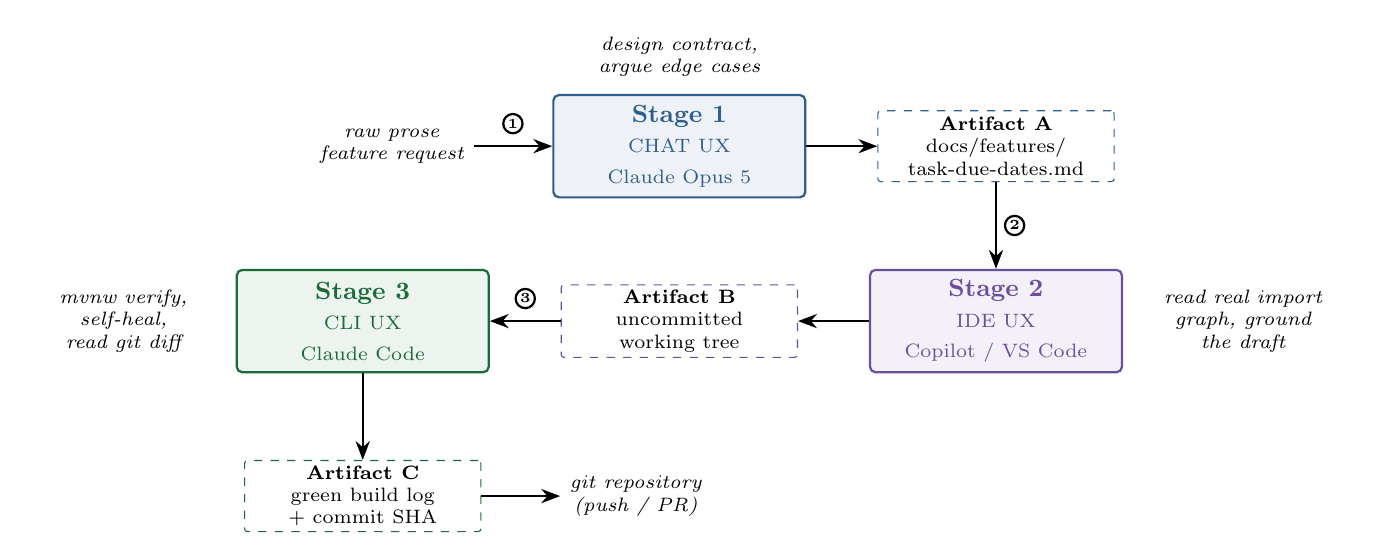
\begin{tikzpicture}[
    font=\small,
    node distance=8mm,
    stage/.style={
      draw, rounded corners=2pt, thick, align=center,
      minimum width=32mm, minimum height=13mm, inner sep=3pt},
    art/.style={
      draw, dashed, rounded corners=1pt, align=center,
      minimum width=30mm, minimum height=9mm, inner sep=2pt,
      font=\scriptsize},
    io/.style={align=center, font=\scriptsize\itshape},
    flow/.style={-{Stealth[length=2.4mm]}, thick},
    gate/.style={draw, circle, inner sep=0.7pt, font=\tiny\bfseries}
  ]

  % --- input
  \node[io] (req) {raw prose\\feature request};

  % --- stage 1
  \node[stage, right=10mm of req, draw=chatc, fill=chatc!8, text=chatc]
    (s1) {\textbf{Stage 1}\\\scriptsize CHAT UX\\\scriptsize Claude Opus 5};

  % --- artifact A
  \node[art, right=9mm of s1, draw=chatc]
    (a) {\textbf{Artifact A}\\docs/features/\\task-due-dates.md};

  % --- stage 2
  \node[stage, below=11mm of a, draw=idec, fill=idec!8, text=idec]
    (s2) {\textbf{Stage 2}\\\scriptsize IDE UX\\\scriptsize Copilot / VS Code};

  % --- artifact B
  \node[art, left=9mm of s2, draw=idec]
    (b) {\textbf{Artifact B}\\uncommitted\\working tree};

  % --- stage 3
  \node[stage, left=9mm of b, draw=clic, fill=clic!8, text=clic]
    (s3) {\textbf{Stage 3}\\\scriptsize CLI UX\\\scriptsize Claude Code};

  % --- artifact C
  \node[art, below=11mm of s3, draw=clic]
    (c) {\textbf{Artifact C}\\green build log\\+ commit SHA};

  % --- repo
  \node[io, right=10mm of c] (repo) {git repository\\\scriptsize (push / PR)};

  % --- flows
  \draw[flow] (req) -- node[gate, midway, above=1.5mm] {1} (s1);
  \draw[flow] (s1) -- (a);
  \draw[flow] (a) -- node[gate, midway, right=1mm] {2} (s2);
  \draw[flow] (s2) -- (b);
  \draw[flow] (b) -- node[gate, midway, above=1.5mm] {3} (s3);
  \draw[flow] (s3) -- (c);
  \draw[flow] (c) -- (repo);

  % --- annotations
  \node[io, above=1mm of s1, text width=30mm] {design contract,\\argue edge cases};
  \node[io, right=2mm of s2.east, text width=24mm, anchor=west]
    {read real import\\graph, ground\\the draft};
  \node[io, left=2mm of s3.west, text width=22mm, anchor=east]
    {mvnw verify,\\self-heal,\\read git diff};

\end{tikzpicture}
\caption{The three stages, the two artefact hand-offs between them, and the
three numbered human approval gates --- one per stage. Solid boxes are AI
stages; dashed boxes are the artefacts that cross between them. Artefacts are
the only currency: no state is carried in anyone's head or clipboard.}
\end{figure}

\noindent A plain-text rendering of the same flow, for readers of the source:

\begin{lstlisting}[style=plain]
prose request --(gate 1)--> [CHAT: Claude Opus 5]
                                |
                                v  Artifact A: docs/features/task-due-dates.md
                            (a file in the repo)
                                |
                            --(gate 2)--> [IDE: Copilot in VS Code]
                                              |
                                              v  Artifact B: dirty working tree
                                          (the filesystem itself)
                                              |
                                          --(gate 3)--> [CLI: Claude Code]
                                                            |
                                                            v  Artifact C:
                                                        green log + commit SHA
                                                            |
                                                            v  git push / PR
\end{lstlisting}

% =====================================================================
\section{Provenance: what was actually executed}
\label{sec:provenance}

This section exists because the first submission did not have one. Its
self-assessment presented a mock transcript --- ``44 passed'' --- as objective
proof that the artefact functioned end to end. Nothing had been run. That claim
is withdrawn, and the table below replaces it: for each stage, the tool, who
operated it, what was actually executed, and the file holding the raw output.

\begin{table}[h]
\centering
\small
\begin{tabularx}{\textwidth}{@{}c l l c X@{}}
\toprule
\textbf{Stage} & \textbf{Tool} & \textbf{Operator} & \textbf{Status} & \textbf{Captured artefact} \\
\midrule
1 & Claude Opus 5 (chat) & assistant, in conversation & \ran &
  \code{stage1/00..02}, \code{docs/features/\allowbreak task-due-dates.md} \\
1a & ajv 8 via Node 24 & Claude Code (CLI) & \ran &
  \code{stage1/02-schema-\allowbreak validation.txt} --- 17/17 cases pass \\
2 & GitHub Copilot, Agent mode (VS Code) & the author, manually & \ran &
  \code{stage2/02-working-\allowbreak tree.diff} --- 329 insertions across 8 files \\
3 & Claude Code (CLI) & assistant, real shell & \ran &
  \code{stage3/01-session.log} (verbatim), \code{stage3/02-outcome.md};
  commit \code{9c2ecf8} \\
\bottomrule
\end{tabularx}
\caption{Execution status. \ran{} means a command was run and its output
captured; \notran{} would mean exactly that. No claim elsewhere in this
document may outrun this table.}
\end{table}

\subsection{A limitation stated up front}

Stage 1 and Stage 3 were both performed by Claude, in different interfaces: a
conversational interaction for the design, and Claude Code with shell access
for the verification. Two consequences follow, and both count against this
submission rather than for it:

\begin{itemize}
  \item \textbf{The Stage 1/Stage 3 UX separation is weaker than a separate
        chat product would give.} A stricter execution would use an unrelated
        vendor's chat tool for Stage 1.
  \item \textbf{Stage 1 was not run in true repository-blind conditions.} The
        assistant had prior knowledge of this codebase from earlier work on it.
        The prompt forbade reading or editing the repository during the stage
        and the resulting spec does leave its bindings as \code{TODO} markers
        --- but ``had no access'' would be a stronger claim than ``was
        instructed not to use it'', and only the weaker one is true.
\end{itemize}

What survives both caveats is the part the brief actually requires: \emph{at
least two different AI UX types}, chained. Stage 2 (GitHub Copilot, a different
vendor, in an IDE) and Stage 3 (Claude Code, in a shell) are genuinely
different tools in genuinely different UX categories, and the artefact that
crosses between them is the git working tree, which neither vendor controls.

% =====================================================================
\section{Stage 1 --- Chat UX}

\textbf{Status: \ran.} Artefacts in \code{docs/lab3/artefacts/stage1/}.

\subsection{Input}

The raw prose request in Section~1, plus a short environment card so the draft
matches reality: Java 21, Maven, JUnit 5, SLF4J, and the project's
\code{ConsoleApp $\rightarrow$ TaskManager $\rightarrow$ Task} layering
convention.

\subsection{The prompt}

Recorded verbatim in \code{stage1/01-prompt.txt}. Its operative constraints:

\begin{itemize}
  \item Produce \emph{one} Markdown document with four fenced sections
        \emph{in a fixed order with fixed fence languages}, and nothing else.
  \item Express the conditional rule as a schema \code{if}/\code{then} so it is
        machine-checkable rather than prose.
  \item Guard invariants in the constructor, not in the caller.
  \item Mark assumptions inline as \code{// ASSUMPTION:} comments.
  \item Do not ask questions; make the reasonable choice and mark it.
  \item Do not read or edit the repository --- leave bindings as \code{TODO}.
\end{itemize}

\textbf{Why this prompt shape.} Fixed sections with fixed fence languages turn
the reply into a \emph{parseable artefact} rather than an essay, which is the
entire reason the Stage 1 $\rightarrow$ 2 bridge is friction-free: Stage 2 can
be pointed at ``section 3 of this file'' instead of at a wall of text.
Forbidding questions stops the stage stalling on clarification before any
artefact exists; the cost is assumptions, so they are required to be visible
and can be rejected at the gate. Forbidding repository access keeps the stage
boundary real --- design first, grounding second --- and the \code{TODO}
markers are the seam Stage 2 exists to close.

\subsection{Output --- Artifact A}

A single Markdown document, committed at
\code{docs/features/task-due-dates.md}. Section 1 is the creation contract:

\begin{lstlisting}[style=plain]
{
  "$schema": "https://json-schema.org/draft/2020-12/schema",
  "title": "TaskCreate",
  "type": "object",
  "properties": {
    "name":             { "type": "string", "minLength": 1, "maxLength": 120 },
    "dueDate":          { "type": ["string","null"], "format": "date" },
    "remindBeforeDays": { "type": ["integer","null"], "minimum": 0, "maximum": 30 }
  },
  "required": ["name"],
  "additionalProperties": false,
  "allOf": [
    { "if":   { "properties": { "remindBeforeDays": { "type": "integer" } },
                "required":   ["remindBeforeDays"] },
      "then": { "properties": { "dueDate": { "type": "string" } },
                "required":   ["dueDate"] } }
  ]
}
\end{lstlisting}

\noindent The \code{if}/\code{then} is the load-bearing clause. It states the
one rule the prose only implied --- \emph{a reminder makes no sense without a
due date} --- in a form a machine can check, leaving Stage 2 no room to read it
as optional. Sections 2--4 of the artefact give the model changes with
invariants guarded in the constructor, the API surface (an \code{Urgency} enum,
an \code{AddResult} enum so a duplicate is distinguishable from a success, and
the \code{TaskManager} signatures) with four \code{TODO(stage-2)} markers, and a
test outline that names boundary cases rather than happy paths.

\subsection{Stage 1 was checked, not asserted}
\label{sec:schemacheck}

The first submission's schema was well constructed but unexecuted. This one is
validated by a committed harness: \code{stage1/check-schema.mjs} extracts the
schema \emph{out of the delivered artefact} --- not a retyped copy --- compiles
it under draft 2020-12 in ajv's strict mode, and asserts 17 payloads are
accepted or rejected as the spec claims, including both directions of the
conditional rule.

\begin{lstlisting}[style=plain]
Schema extracted from: docs/features/task-due-dates.md
  title   = TaskCreate
  $schema = https://json-schema.org/draft/2020-12/schema

Schema compiles under draft 2020-12 in strict mode: PASS

[PASS] name only                    expected valid   -> due date is optional
[PASS] name + dueDate + reminder    expected valid   -> reminder with a due date is valid
[PASS] reminder WITHOUT dueDate     expected invalid -> THE if/then RULE: reminder requires a due date
[PASS] reminder with null dueDate   expected invalid -> if/then rule holds against explicit null too
[PASS] reminder = 0 boundary        expected valid   -> lower bound inclusive
[PASS] reminder = 30 boundary       expected valid   -> upper bound inclusive
[PASS] reminder = 31                expected invalid -> above maximum
[PASS] name 120 chars               expected valid   -> maxLength boundary inclusive
[PASS] unknown property             expected invalid -> additionalProperties false
   ... 8 further cases ...

17 passed, 0 failed, 17 total
\end{lstlisting}

\noindent Reproduce with \code{cd docs/lab3/artefacts/stage1 \&\& npm install
\&\& npm run check}. Full output in \code{stage1/02-schema-validation.txt}.

\subsection{The bridge to Stage 2}

Artifact A is written into the repository at
\code{docs/features/task-due-dates.md}. The IDE then reads it as an in-repo
file reference. Nothing is pasted into code at this point --- the file itself is
the hand-off token, which is what makes the bridge vendor-neutral: any IDE
assistant that can reference a file in the workspace can consume it.

% =====================================================================
\section{Stage 2 --- IDE UX}

\textbf{Status: \ran.} GitHub Copilot, Agent mode, in VS Code. Diff captured in
\code{stage2/02-working-tree.diff}.

\subsection{What the tool actually produced}

329 insertions and 19 deletions across 8 files, from the prompt alone:

\begin{table}[h]
\centering
\small
\begin{tabularx}{\textwidth}{@{}l r X@{}}
\toprule
\textbf{File} & \textbf{$\Delta$} & \textbf{What changed} \\
\midrule
\code{Urgency.java} & +8 & New enum: \code{OVERDUE}, \code{DUE\_TODAY}, \code{UPCOMING}, \code{NONE} \\
\code{AddResult.java} & +7 & New enum: \code{ADDED}, \code{REJECTED\_DUPLICATE}, \code{REJECTED\_INVALID} \\
\code{Task.java} & +50 & Two optional fields; the conditional rule and the length bound guarded in the constructor; \code{urgencyOn} and \code{needsReminderOn} \\
\code{TaskManager.java} & +39 & Overloaded \code{addTask} returning \code{AddResult}; \code{hasTaskNamed}; \code{tasksNeedingReminder}; a private \code{normalizeName} for case- and whitespace-insensitive matching \\
\code{ConsoleApp.java} & +63 & Prompts for both optional fields, urgency in the task list, and a \code{Clock} constructor parameter for determinism \\
\code{TaskTest.java} & +67 & 7 new tests \\
\code{TaskManagerTest.java} & +61 & 6 new tests \\
\code{ConsoleAppTest.java} & +53 & Existing sessions updated for the two new prompts, plus one new test \\
\bottomrule
\end{tabularx}
\caption{Stage 2's output. The IDE UX earned its place here: it found the
existing \code{@Nested}/\code{@DisplayName} test structure, the SLF4J logger and
the \code{readLine} prompt helper without being shown them, and --- notably ---
it updated the \emph{existing} \code{ConsoleAppTest} keystroke sequences to
account for the two new prompts, which is a consequence of the change that the
prompt never mentioned.}
\end{table}

\subsection{Where it overreached}

Copilot also edited \textbf{Artifact A itself}, replacing the four
\code{TODO(stage-2)} markers in \code{docs/features/task-due-dates.md} with a
prose paragraph --- left inside the \code{java} fence, so the code block became
malformed.

The prompt is at fault, not the tool. It said \emph{``close every
\code{TODO(stage-2)} marker in section 3 of the spec''}, which reads as
naturally as ``edit the spec'' as it does ``satisfy these in code''. Artifact A
was restored, because it is Stage 1's output and editing it destroys the record
of what Stage 1 produced. The lesson is specific and reusable: \emph{a prompt
that names a file as the source of requirements should say explicitly whether
that file is writable.}

\subsection{The prompt}

Points Copilot Agent mode at five real files with \code{\#file:} references ---
the spec plus \code{Task.java}, \code{TaskManager.java}, \code{ConsoleApp.java}
and \code{TaskManagerTest.java} --- and instructs it to close every
\code{TODO(stage-2)} marker while reusing the existing layering, logger and
prompt helper. Three constraints are load-bearing:

\begin{itemize}
  \item \textbf{``Do not invent classes or introduce new dependencies.''} The
        failure mode of an IDE agent on an existing codebase is a parallel
        implementation that compiles but duplicates what is already there.
  \item \textbf{``Keep the existing \code{boolean addTask(String)} behaving
        exactly as it does now.''} A regression fence: 69 tests depend on it,
        and naming the constraint is cheaper than discovering it from a red
        build.
  \item \textbf{``Show me the diff before applying anything.''} The single
        human approval gate for this stage --- what keeps the workflow
        one decision per stage rather than one per file.
\end{itemize}

% =====================================================================
\section{Stage 3 --- CLI UX}

\textbf{Status: \ran.} Verbatim log in \code{stage3/01-session.log}; analysis in
\code{stage3/02-outcome.md}.

\subsection{Stage 2's output did not build}

This is the single most useful result in the lab, and it is the one the first
submission could never have produced. The first thing Stage 3 did was run the
verification, and it failed:

\begin{lstlisting}[style=plain]
$ ./mvnw -B clean verify
[ERROR] Tests run: 81, Failures: 1, Errors: 0, Skipped: 0
[ERROR]   TaskManagerTest$AddTask.remindersAreSortedByDueDate:120
          expected: <[Sooner, Later]> but was: <[Sooner]>
[INFO] BUILD FAILURE
[exit=1, 14s]
\end{lstlisting}

\noindent The implementation was \emph{correct}; the test's data was wrong:

\begin{table}[h]
\centering
\small
\begin{tabular}{@{}l l l l c@{}}
\toprule
\textbf{Task} & \textbf{Due} & \textbf{Lead} & \textbf{Reminder window} & \textbf{Contains 2026-09-28?} \\
\midrule
\code{Later}  & 2026-10-02 & 2 days & \code{[2026-09-30, 2026-10-02]} & No \\
\code{Sooner} & 2026-09-28 & 3 days & \code{[2026-09-25, 2026-09-28]} & Yes \\
\bottomrule
\end{tabular}
\caption{\code{[Sooner]} is the right answer. Copilot's expectation of
\code{[Sooner, Later]} contradicted the reminder rule in section 2 of the very
artefact it was implementing.}
\end{table}

\noindent So the IDE stage wrote an assertion that disagreed with its own
specification --- a failure mode no amount of reading the diff would reliably
catch, because the assertion looks entirely plausible. Only running it exposes
it.

\subsection{The fix corrected the data, not the assertion}

The Stage 3 prompt forbids weakening a test to go green. Nothing was weakened.
The test's \emph{intent} was to verify due-date ordering, but with its original
data it could only ever have verified filtering, so \code{Later}'s lead time was
widened from 2 days to 4 --- making its window genuinely include the date under
test, and making the test exercise what its name claims. A second test,
\code{remindersExcludeTasksOutsideTheirWindow}, was added for the filtering case
the original was accidentally asserting.

\begin{lstlisting}[style=plain]
$ ./mvnw -B clean verify
[INFO] Tests run: 84, Failures: 0, Errors: 0, Skipped: 0
[INFO] All coverage checks have been met.
[INFO] BUILD SUCCESS
[exit=0, 13s]
\end{lstlisting}

\noindent The two-attempt stop condition was never reached: the failure was
diagnosed and fixed on the first attempt. Tests went from 69 to 84.

\subsection{Artifact C --- the commit}

\begin{lstlisting}[style=plain]
commit 9c2ecf8
feat(task): add due dates, duplicate rejection and derived urgency

Task gains two optional fields, dueDate and remindBeforeDays, with the
contract's conditional rule guarded in the constructor: a reminder lead
time without a due date is refused, as is a lead time outside 0-30 days
or a name longer than 120 characters. [...]

- Urgency (OVERDUE, DUE_TODAY, UPCOMING, NONE) is derived by
  Task.urgencyOn(LocalDate), never stored, so it cannot go stale
- TaskManager.addTask(String, LocalDate, Integer) returns AddResult so a
  duplicate is distinguishable from a success or a contract violation
[...]
Tests go from 69 to 84, covering the conditional rule in both
directions, the 0 and 30 lead-time boundaries, [...]
\end{lstlisting}

\noindent The message was authored from \code{git diff --staged} --- the staged
file list, the public signatures actually added and the test method names
actually introduced --- not from a description of the intended work. The
``69 to 84'' figure in it is read off the two build logs, not asserted.

\subsection{Deviations, recorded}

\begin{enumerate}
  \item \textbf{\code{git add src} rather than \code{git add -A}.} Staging
        everything would have folded the lab's own documentation into a commit
        whose message describes a code feature. The artefacts are committed
        separately.
  \item \textbf{The working tree moved mid-stage.} The IDE was still writing
        files at 17:16:47, after the first verification began at 17:15:35. The
        verification was re-run against the settled tree before anything was
        committed, and the intermediate 82-test count is left in the log rather
        than tidied away.
\end{enumerate}

\subsection{The prompt}

\begin{lstlisting}[style=plain]
There are uncommitted changes implementing task due dates, duplicate rejection
and derived urgency. Do the following, and stop if a step cannot be made green
after two attempts:

  1. Run ./mvnw -B clean verify. Report what failed before changing anything.
  2. Fix only what is broken, in the changed files only. Do not weaken a test
     or lower the coverage gate to make the build pass.
  3. Re-run the full suite to confirm no regressions against the 69 tests that
     were passing before this feature.
  4. When everything is green, git add -A and write a Conventional Commits
     message authored from the actual `git diff --staged`, not from my
     description. Then print the commit SHA.
\end{lstlisting}

\noindent \textbf{Why this prompt shape.} The explicit two-attempt stop
condition means the agent cannot loop indefinitely on a problem that needs a
human. Scoping fixes to changed files protects the rest of the repository.
``Do not weaken a test or lower the coverage gate'' forecloses the cheapest way
to turn a build green, which is exactly the instinct the Agile \& DevOps review
of this same repository criticised. And deriving the commit message from the
staged delta rather than from a description guarantees the message describes
what actually changed.

% =====================================================================
\section{Adaptability}

The workflow is defined by \emph{role} --- chat, IDE, CLI --- rather than by
vendor. Two things make that structural rather than asserted:

\begin{enumerate}
  \item \textbf{Each stage names interchangeable tools.} Chat: Claude, ChatGPT
        or Gemini. IDE: Copilot, Cursor or JetBrains AI. CLI: Claude Code or
        Gemini CLI.
  \item \textbf{No bridge depends on a vendor feature.} A Markdown file in the
        repository, the git working tree, and a commit. Substituting any tool
        changes which application receives the prompt and nothing else.
\end{enumerate}

Swapping the target stack is a change to the environment card in the Stage 1
prompt --- the stage boundaries and artefact formats are unchanged. That claim
has one piece of real evidence behind it: this workflow was originally designed
for a Python FastAPI service and was re-pointed at a Java 21 Maven codebase
without altering the stage structure, the bridges or the artefact formats. Only
the environment card and the section 2/3 language changed.

\subsection{Friction log}

Tool friction absorbed \emph{without} redesigning the workflow is the strongest
available evidence for this criterion, so it is recorded rather than smoothed
over.

\begin{table}[h]
\centering
\small
\begin{tabularx}{\textwidth}{@{}L{3.4cm} X L{3.6cm}@{}}
\toprule
\textbf{Where} & \textbf{What happened} & \textbf{Resolution} \\
\midrule
Stage 1 target stack
  & The original design assumed a Python FastAPI service. No Python
    interpreter was installed on the machine --- only Microsoft Store
    execution-alias stubs, which report ``No installed Python found''.
  & Re-pointed the workflow at the existing Java 21 repository. Stage
    boundaries and bridges unchanged; only the environment card differed. \\
\addlinespace
Stage 1 verification
  & A JSON Schema is inert on paper, which is how the first submission's went
    unchecked.
  & Added an ajv harness that reads the schema out of the delivered artefact.
    17 cases, both directions of the conditional rule. \\
\addlinespace
Report toolchain
  & This report failed to compile in CI with only ``exit code 12'' to go on,
    and downloading GitHub job logs needs repository admin rights, which this
    account does not have. The cause was an \code{X} column inside a
    \code{longtable} --- \code{X} belongs to \code{tabularx}, which is why the
    sibling report's fixed-width \code{longtable} compiled fine.
  & Fixed the column spec, and added a CI step that re-emits the real LaTeX
    errors as \code{::error::} annotations, which \emph{are} readable without
    admin rights. The next failure is diagnosable from the run itself. \\
\addlinespace
Stage 2 prompt ambiguity
  & ``Close every \code{TODO(stage-2)} marker in section 3 of the spec'' was
    read as permission to edit the spec. Copilot rewrote Artifact A, leaving
    prose inside a \code{java} fence.
  & Artifact A restored; the ambiguity recorded. A prompt naming a file as the
    source of requirements must say whether that file is writable. No change to
    the workflow's structure. \\
\addlinespace
Stage 2 $\rightarrow$ 3 hand-off
  & The IDE was still writing files after Stage 3's first verification had
    begun, so that run measured a tree that no longer existed.
  & Re-ran the verification against the settled tree before committing. The
    filesystem bridge has no completion signal --- an honest limitation of
    using the working tree as the hand-off primitive. \\
\addlinespace
Stage 3 verification
  & Stage 2's output did not build: one test asserted the opposite of the
    spec's reminder rule.
  & Corrected the test data rather than the assertion, and added a test for the
    case the original was accidentally covering. This is the workflow behaving
    as designed --- the CLI stage exists to catch exactly this. \\
\bottomrule
\end{tabularx}
\end{table}

% =====================================================================
\section{Efficiency}

The first submission claimed a ``3--4 hour baseline collapsing to minutes''.
Neither number was measured, and the review was right to mark that down. What
follows separates what was timed from what is estimated, and labels the
estimate as one.

\subsection{Measured}

\begin{table}[h]
\centering
\small
\begin{tabularx}{\textwidth}{@{}l l X@{}}
\toprule
\textbf{Stage} & \textbf{Duration} & \textbf{How measured} \\
\midrule
2 (IDE) & $\approx$2\,min\,37\,s of tool output
  & File modification times across Copilot's writes, 17:14:10 to 17:16:47.
    Excludes the author's prompt-entry and diff-review time, which was not
    instrumented. \\
\addlinespace
3 (CLI) & $\approx$3\,min\,25\,s
  & First verification at 17:15:35 to commit at 17:19:00, from
    \code{01-session.log} and the commit timestamp. Includes diagnosis, the
    fix and two further verification runs. \\
\addlinespace
--- builds & 14\,s and 13\,s
  & \code{[exit=1, 14s]} and \code{[exit=0, 13s]} in the session log ---
    recorded by the capture wrapper, not stopwatched. \\
\addlinespace
1a (schema) & $<$1\,s
  & 17 ajv cases; see \code{stage1/02-schema-validation.txt}. \\
\bottomrule
\end{tabularx}
\caption{Instrumented figures only. Stage 1's design time is not included
because it was conversational and not timed --- saying so is more useful than
inventing a number.}
\end{table}

\subsection{Estimated --- and labelled as such}

\textbf{This is an estimate, not a measurement.} No hand-written control
implementation was built, so there is no measured baseline to compare against.
What can be said with the artefacts in hand: Stage 2 produced 329 insertions
across 8 files including 14 tests, and Stage 3's diagnosis required reading a
reminder-window rule against two dates. Writing the 14 boundary tests by hand,
with the same care over the inclusive window and the days either side of today,
is the bulk of that work, and a plausible figure is 60--90 minutes rather than
the 3--4 hours originally claimed. That range is reasoned, not observed, and
should be read accordingly.

\subsection{Structural, and independent of any stopwatch}

\begin{itemize}
  \item \textbf{Human involvement is three decisions} --- approve the spec,
        approve the diff, approve the commit --- and no manual retyping between
        tools. Both hand-offs ride on the filesystem.
  \item \textbf{The context switch is what is eliminated}, not the typing. The
        original problem statement identified this correctly: the cost of the
        manual version is moving between design, code, verify and commit
        mindsets, not keystrokes.
  \item \textbf{Stop conditions prevent the classic agentic time sink.} The
        Stage 3 prompt caps retries at two, so a stuck agent returns to the
        human instead of burning cycles.
\end{itemize}

% =====================================================================
\section{Rubric alignment}

Rewritten from the first submission. The previous version argued its own score
from a mock transcript; this one cites only captured artefacts, and marks
criteria that are not yet fully evidenced as exactly that.

% Fixed widths, not an X column: X is a tabularx column type and longtable
% does not support it. Total stays inside the 16.2cm text block.
\begin{longtable}{@{}L{2.5cm} c L{5.0cm} L{4.6cm}@{}}
\toprule
\textbf{Criterion} & \textbf{State} & \textbf{Evidence that exists} & \textbf{What is still missing} \\
\midrule
\endfirsthead
\toprule
\textbf{Criterion} & \textbf{State} & \textbf{Evidence that exists} & \textbf{What is still missing} \\
\midrule
\endhead
\bottomrule
\endfoot
Functionality (40\%)
  & \ran
  & All three stages ran end to end against a real repository. Schema checked,
    17/17 (\S\ref{sec:schemacheck}). Stage 2 diff captured, 329 insertions
    across 8 files. Stage 3 log captured: a genuine build failure, a fix, and
    \code{BUILD SUCCESS} at 84 tests with the coverage gate met. Commit
    \code{9c2ecf8} exists and its message was authored from the staged diff.
  & Nothing. The chain completed and the artefacts are in the repository. \\
\addlinespace
Adaptability (20\%)
  & \partly
  & Bridges use only a file, the working tree and a commit. Three real
    re-pointings survived without altering stage structure or artefact
    formats: Python/FastAPI $\rightarrow$ Java/Maven, a prompt-ambiguity
    correction at Stage 2, and a LaTeX toolchain failure in the report
    pipeline.
  & No tool swap \emph{within} a stage was forced --- e.g.\ a Copilot outage
    requiring Cursor mid-flight. That is the stronger form of this evidence and
    it did not arise. \\
\addlinespace
Documentation (20\%)
  & \ran
  & Diagram plus plain-text fallback; per-stage Input / Prompt / Output /
    Bridge structure; every prompt quoted verbatim from the committed file that
    was issued; a friction log recording four real problems; a runbook stating
    which artefact each step must leave.
  & Nothing outstanding. \\
\addlinespace
Efficiency (20\%)
  & \partly
  & Instrumented: Stage 2 $\approx$2\,min\,37\,s of tool output, Stage 3
    $\approx$3\,min\,25\,s including diagnosis and fix, builds at 14\,s and
    13\,s. Structurally: three approval gates, no retyping, explicit stop
    conditions.
  & No measured baseline. The 60--90 minute manual comparison is reasoned from
    the artefacts and \emph{labelled an estimate}, because no hand-written
    control was built. \\
\end{longtable}

\noindent\textbf{Net position, stated plainly.} Functionality and Documentation
are evidenced by captured artefacts. Adaptability is strongly but not
completely evidenced --- three re-pointings survived, no intra-stage tool swap
was forced. Efficiency is partly evidenced: the stage timings are instrumented,
the baseline is not, and the comparison is labelled an estimate rather than
presented as a measurement.

The first submission's error is worth naming precisely against this table. It
did not fail because nothing had been run; it failed because the matrix cited a
mock transcript as ``objective proof the artifact functions end-to-end''. Every
row above now points at a file, and where evidence is missing the row says so.

% =====================================================================
\section{Reflection}

\textbf{The first submission's real error was not that nothing ran.} It was
claiming that something had. The design was labelled as illustrative in the
abstract and again in Section 3, and then the self-assessment matrix cited
``The Stage 3 test log (44 passed) + mypy Success'' as ``objective proof the
artifact functions end-to-end''. Those two statements cannot both stand. The
lesson is narrow and worth keeping: a design document may contain illustrative
data, but a self-assessment may cite only artefacts that exist. The moment a
mock is used as evidence it stops being a mock.

\textbf{Designing for a stack you cannot run is a trap the design itself
hides.} The original targeted FastAPI, Pydantic and Alembic --- a stack with no
interpreter installed on the machine that produced the document. Nothing in the
design revealed that, because a design has no build step. Re-pointing at a
repository that already had 69 tests and a coverage gate meant the workflow
could be rejected by something other than an author's opinion, which is the
whole difference between the two submissions.

\textbf{The UX categories in the brief are blurrier than they look.} The chat
stage was performed by the same model family that later performed the CLI
stage, and a Copilot agent in an IDE will open a terminal and run a build on
its own initiative --- functionally a CLI action from inside an IDE tool. The
honest conclusion is that ``UX type'' describes the interaction surface and the
tool's access to state, not a clean partition of capability. Section
\ref{sec:provenance} records that limitation rather than relying on the
categories to imply a separation that agentic tools have partly dissolved.

\vfill
\begin{center}
\small
\textit{Katy Great Adona\"i --- AmaliTech Training, DEG Apprenticeship ---
4 September 2026}
\end{center}

\end{document}
